\chapter{Design-Time Network Performance Analysis of Distributed CPS Applications}
\label{ch:designTime}

In this chapter, we describe research results related to the
challenge of accurately predicting network QoS for systems which may
require strict guarantees about performance and resource utilization.

\iffalse
Networking often performs a key role in CPS, such as facilitating
the communication and control of distributed sensors and control
systems.  Traditionally, these networks of CPS have been both isolated
from external influences and predefined at system design-time.  This
isolation and pre-determination creates a static network with respect
to both the topology of the network and the capacity of each network
link.  More recently however, CPS have become less isolated and more
dynamic by utilizing heterogeneous and wireless networks and
incorporating mobility.  Such systems include wireless sensor networks
(WSN), mobile ad-hoc networks (MANETs), and distributed real-time
embedded systems (DRES).  These types of systems are being developed
to provide remote sensing and control capabilities, smart grid and
smart city infrastructure, and smart vehicle communications networks,
to name a few.
\fi

Analyzing application and system network Quality of Service (QoS)
requires either design-time models and analysis techniques or
experimental measurements from an application and system testbed.  For
high- or mixed-criticality software and systems, typically
experimental measurements are used but often these can be incomplete
or quite costly to generate.  Instead, a design-time modeling paradigm
for networked applications and systems can provide developers and
system integrators the information to accurately predict the system
and application network QoS.

\begin{figure}[ht!]
  \centering
  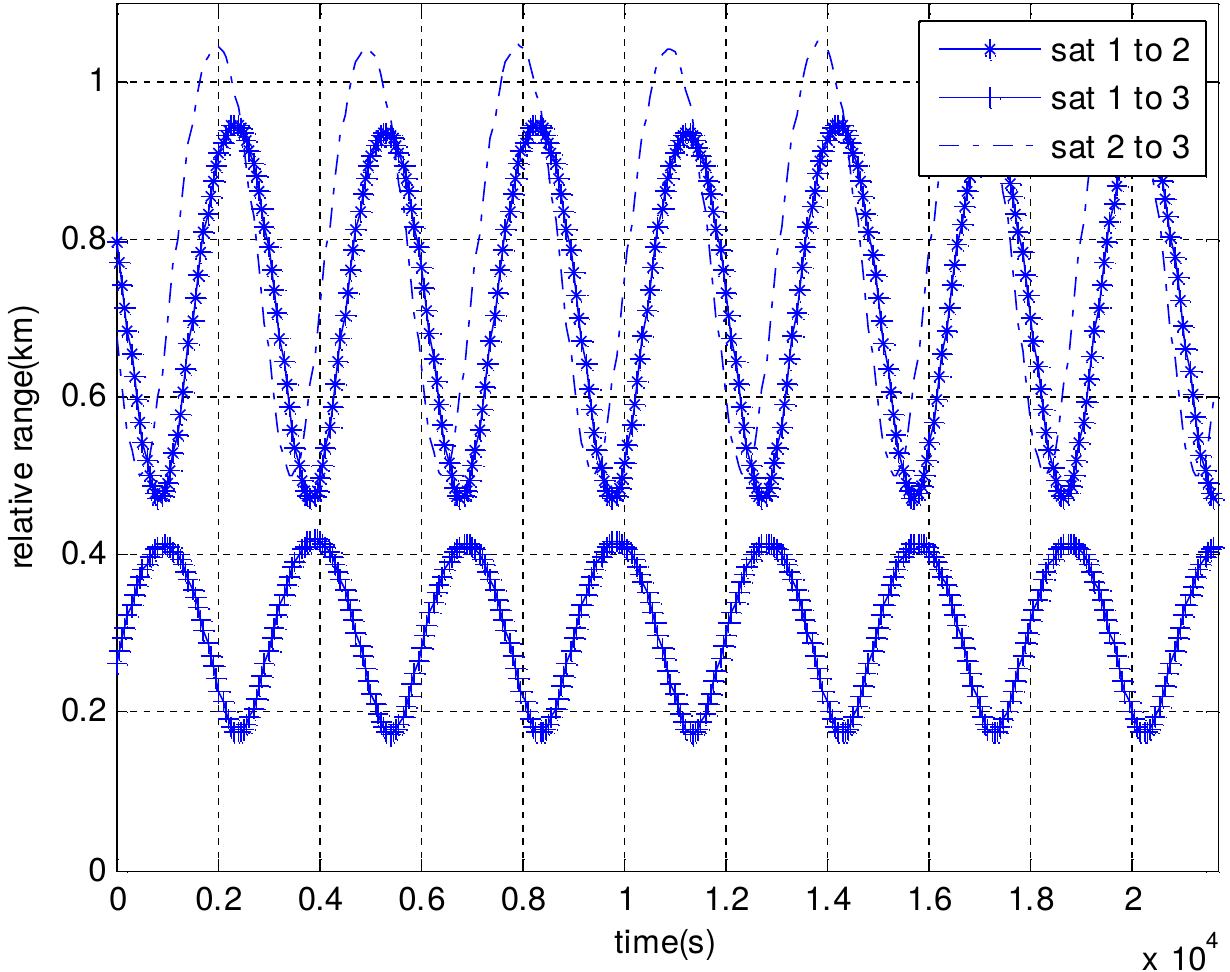
\includegraphics[width=0.85\textwidth]{figs/cluster_distance.png}
  \caption{Distance as a function of time (pairwise) between
    satellites in a cluster orbiting Earth.  The network capacity
    varies for each network link between two satellites inversely
    proportional to the distance between them.  Reprinted from
    \cite{satellite_distance}.}
  \label{fig:satellite_network}
\end{figure}

Some wireless mobile CPS networks, such as the network between a
cluster of satellites orbiting Earth, vary periodically with respect
to time, \emph{e.g.} according to the cluster's orbital period.  An
example of such periodic variation in satellite network capacity is
shown in Figure~\ref{fig:satellite_network}.  For such networks, the
physical dynamics of the nodes in the cluster are well understood and
predictable, therefore the network dynamics can be fairly predictable
as well.  For such predictable or periodic dynamic networks, the use
of worst-case network performance for analysis and constraint
verification wastes the network resources over much of the life-cycle
of the system. Integrating the physical dynamics of the network into
the modeling and analysis tools improves the performance of the
systems without degrading its reliability.

%%%%%%%%%%%%%%%%%%%%%%%%%%%%%%%%%%%%%%%%%%%%%%%%%%%%%%%%%%%%%%%%%%%%%%%%%%%%%%%%%%%
%%%%%%%%%%%%%%%%%%%%%%%%%%%%%%%%%%%%%%%%%%%%%%%%%%%%%%%%%%%%%%%%%%%%%%%%%%%%%%%%%%%
%%%%%%%%%%%%%%%%%%%%%%%%%%%%%%%%%%%%%%%%%%%%%%%%%%%%%%%%%%%%%%%%%%%%%%%%%%%%%%%%%%%
%%%%%%%%%%%%%%%%%%%%%%%%%%%%%%%%%%%%%%%%%%%%%%%%%%%%%%%%%%%%%%%%%%%%%%%%%%%%%%%%%%%
%%%%%%%%%%%%%%%%%%%%%%%%%%%%%%%%%%%%%%%%%%%%%%%%%%%%%%%%%%%%%%%%%%%%%%%%%%%%%%%%%%%
\section{Precise Modeling of Application Network Traffic and System Network Resources for Performance Prediction}
\label{sec:framework} 

To precisely predict network performance for applications distributed
in a mobile CPS, we need precise models of both the application
network resource requirements and the system's network resource
capacity.  These predictions, if precise and reliable enough, can
serve as guarantees for application developers and system integrators
about the network QoS that the system will provide and the network
resources the application will receive.

\subsection{Problem}
Current design tools do not incorporate the physical dynamics of the
network for analysis of network constraints on the applications. For
systems with known models of system dynamics, the system's dynamics
should be incorporated into the modeling tool and should integrate
with the other models of the system, e.g. the system's network models.
Because of the diversity of CPS, IoT systems, and other networked
embedded systems in general, modeling and analysis tools targeted
towards these systems must support a wide range of configurations,
architectures, standards, and interfaces.  The same compatibility is
required in network modeling and analysis frameworks.  Because many of
these systems may support different types of network communications
hardware, often using multiple types of network interface hardware
within the same system, the models of the network must be able to
express network resources in a way that can capture these differences.
Because of this diversity and the modeling semantics of the commonly
used paradigms (e.g. Real-Time Calculus), developing very precise
predictions is difficult, since the models are not very precise with
respect to the actual behavior of the applications on the system.

\subsection{Mathematical Formalism}
\label{subsec:math_formalism}

To model the network capability of the system and the application
traffic patterns, we have developed a network modeling paradigm
similar to Network Calculus' traffic arrival curves and traffic shaper
service curves.  This paradigm is called \fulltool/ (\shorttool/). 

Similarly to Network Calculus' arrival curves and service curves, our
network profiles model how the system's network performance or
application traffic generation changes with respect to time.  Whereas
Network Calculus' modeling transforms application data profiles and
network service profiles into max/min curves for data
received/serviced vs. length of time-window, our models take a simpler
approach which models exactly the data generated by the application
and the data which could be sent through the network, allowing our
performance metrics to be more precise.  Specifically, the bandwidth
that the network provides on a given communication link is specified
as a periodic time series of scalar bandwidth values. Here, bandwidth
is defined as data rate, i.e. bits per second, over some averaging
interval.  This bandwidth profile can then be time-integrated to
determine the maximum amount of data throughput the network link could
provide over a given time.  The bandwidth profile for the application
traffic similarly can be time-integrated to determine the amount of
data that the application attempts to send on the network link as a
function of time.

Having time-integrated the bandwidth profiles to obtain data vs. time
profiles that the application requires and that the system provides,
we can use a special type of convolution ($\otimes$),
\emph{(min,+)-calculus convolution}, on these two profiles to obtain
the transmitted link data profile as a function of discrete time. The
convolution we define on these profiles borrows concepts from the
min-plus calculus used in Network Calculus, but does not use a
sliding-window and instead takes the transformed minimum of the
profiles. For a given application data generation profile, $r[t]$, and
a given system link capacity profile $p[t]$, where $t\in\mathbb{N}$,
the link transmitted data profile $l[t]$ is given by the convolution
Equation~\ref{eq:convolution}. The difference $(p[t-1] - l[t-1])$
represents the difference between the amount of data that has been
transmitted on the link $(l[t-1])$ and the data that the link could
have transmitted at full utilization $(p[t-1])$. As demonstrated by
the convolution equation, $\forall t : l[t] \le r[t]$, which is the
relation that, without lower-layer reliable transport, the link cannot
transmit more application data for the application than the
application requests.  Note that there will be packetization and
communication header overhead which will be transmitted with
application data.  The overhead can be determined at design time and
can therefore be accounted for in the application profile.

\begin{equation}
	\label{eq:convolution}
	\begin{split}
		y=l[t] &= (r \otimes p)[t] \\ &= min( r[t] , p[t] -
                (p[t-1] - l[t-1]) )
	\end{split}
\end{equation}

\begin{align}
	\label{eq:buffer}
	&\text{buffer}= sup\{r[t] - l[t] : t \in \mathbb{N}\}\\
	\label{eq:delay}
	&\text{delay} = sup\{l^{-1}[y]-r^{-1}[y] : y \in \mathbb{N}\}
\end{align}

\begin{figure}[h!]
	\centering
        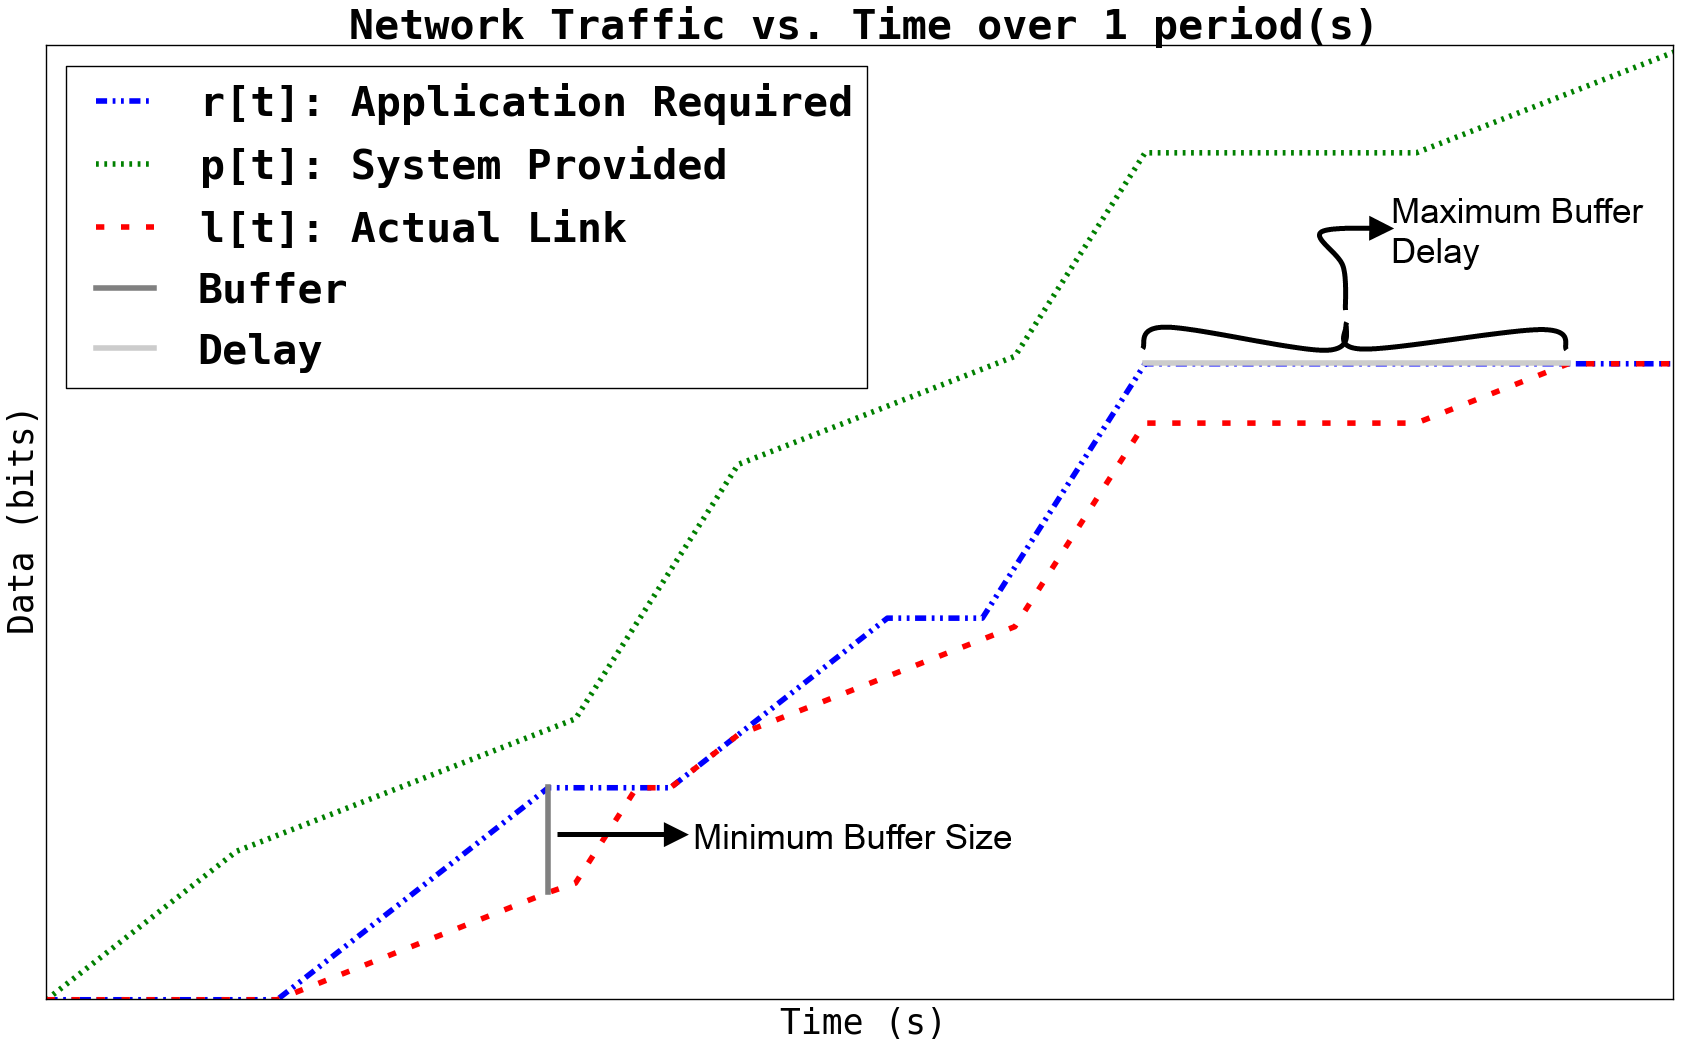
\includegraphics[width=0.85\textwidth]{figs/convolution6.png}
	\caption{Representative example demonstrating convolution of
          the data vs. time profiles that the application requires and
          that the system provides.  The resultant data vs. time
          profile describes the data that the system actually
          output onto the link.}
	\label{fig:convolution}
\end{figure}

Equation~\ref{eq:buffer} and Equation~\ref{eq:delay} calculate, using
$l[t]$, $r[t]$, and the inverse function $l^{-1}[y]$, the minimum
buffer size required for the application and the maximum buffering
delay experienced by application data, respectively.
Figure~\ref{fig:convolution} depicts the convolution operation and
shows a schematic representation of the maximum buffer delay and the
minimum buffer size.  As can be seen in the figure, the maximum
horizontal distance between the required profile and the link profile
is equal to the maximum buffer delay, while the maximum vertical
distance is equal to the minimum buffer size required for loss-less
transmission of data on the link.

We developed the \shorttool/ paradigm to precisely
model system network resources as they vary with respect to time.
Similarly, the application network resource requirements can be
modeled very precisely as functions of time.  These models can be more
precise than the models developed for Network Calculus since they are
explicitly functions of time, instead of functions of time-windows.
Taking the example from earlier, a bulk data transfer (BDT) initiated
from the satellite cluster to a ground station is scheduled for when
the satellite cluster is within range of the ground station and
therefore has a good downlink to the ground.  With our paradigm, this
coupling between the network traffic flow and the network resource
availability can be captured explicitly in the model.  Under the
Network Calculus modeling semantics however, such a BDT would
negatively affect the predicted required network buffer size and
network buffering latency since that BDT data transmission window
(i.e. the window of time it sends the data on the link) would be
compared against the minimum service provided by the network to the
ground station (which would be zero during the parts of the orbit when
the ground stations are not within range of the cluster).  Such a
comparison drastically increases the predicted buffer space required
and predicted buffering latency incurred by the BDT data.

This network modeling and analysis technique we developed has been
reported in \cite{ISIS_F6_CYPHY:14}, which describes the network
resource models, their composition, and the calculation of performance
metrics such as buffer requirements and buffering delay.

\subsection{Accuracy and Precision}
\label{subsec:precision}

When developing a new analysis technique to predict application
network performance, verification that the results of the analysis are
accurate is paramount.  Experimental results are required not only to
judge whether or not the theory is sound, but also to allow
application developers and system integrators to judge the
applicability of the analysis to their systems and applications.  If
the error in the predicted performance metrics is too high, the
analysis results will cease to be useful.

To verify the validity of these operations and metrics, we developed
network measurement code which produced data for the network according
to the supplied profile.  This code executed on a private network
testbed of nodes connected to each other through a gigabit Ethernet
switch. We emulated the network link profile using traffic shaping in
the Linux kernel's traffic control (TC)\cite{linux_tc}, which can be
configured to control bandwidth, latency, and packet loss.  For these
experiments, we configured the traffic shaping to control the data
rate of the application data on the network interface according to the
system provided network profile.

On this testbed we ran application network traffic producer code which
produces network traffic according to the supplied application
profile.  The profiles for the application and system are shown in
Figure~\ref{fig:experimental_validation}.  This traffic producer code
measured the delay, throughput, and buffer requirements of the traffic
that was produced.  By collecting these measurements over the course
of multiple tests, we measured the differences between the predicted
and measured buffer size and delay.  The accuracy of our prediction
was reported in \cite{ISIS_F6_CYPHY:14} and is shown in
Table~\ref{table:results}.

\begin{figure}[ht!]
  \centering
  \subfigure[System Data Rate vs. Time]{
    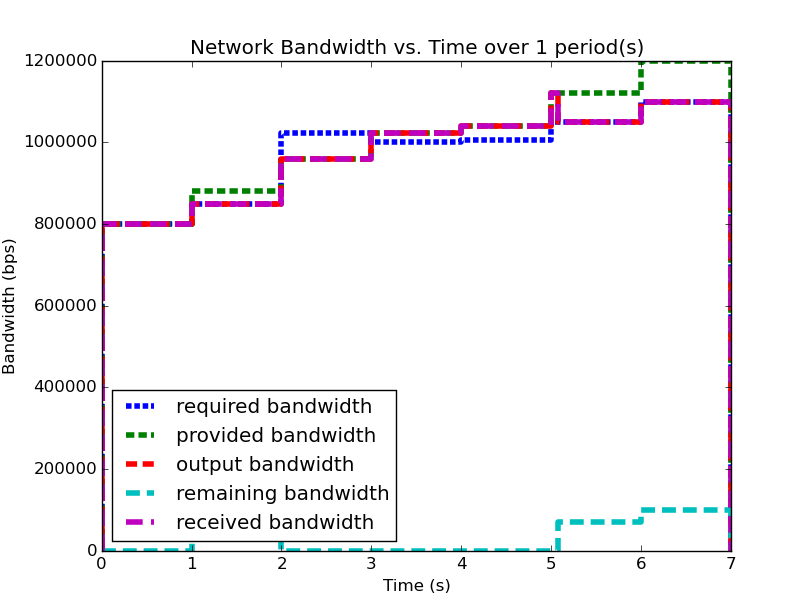
\includegraphics[width=0.8\textwidth]{../doc/src/images/results/maren_namek_bw.png}
  }
  \subfigure[System Data Analyzed with \shorttool/]{
    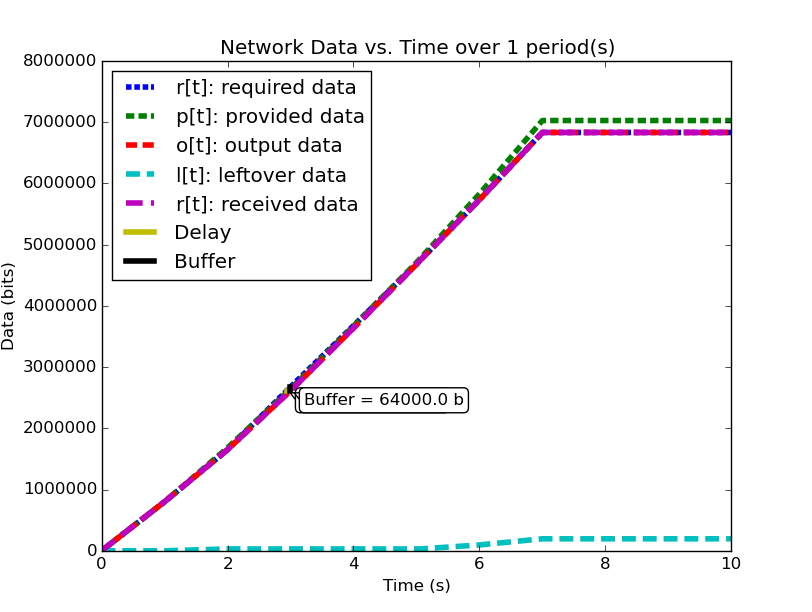
\includegraphics[width=0.8\textwidth]{../doc/src/images/results/maren_namek_data.png}
    \label{subfig:pnp_analysis_comparison}
  }
  \caption{System and application profiles used for experimental
    validation of \shorttool/. The Analysis using \shorttool/ is
    shown on the right.}
  \label{fig:experimental_validation}
\end{figure}

\begin{table}[htbp]
\caption{Network utilization calculations and measured results using UDP over IPv6.}
\begin{tabular}{| c | c | c |}
\hline
 & Predicted & Measured ($\mu,\sigma$) \\\hline
Buffer Delay (s) & 0.0625 & (0.06003 , 0.00029) \\\hline
Time of Delay (s) & 3.0 & (2.90547 , 0.00025) \\\hline
Buffer Size (bytes) & 8000 & (7722.59 , 36.94) \\\hline
\end{tabular}
\label{table:results}
\end{table}

As can be seen in the table, the predictions made by our analysis
techniques are tight, conservative bounds on the actual performance of
the application in the experimental system.  Both the predicted delay
and the predicted buffer size required for the application were less
than 10 percent different from the actual system's required buffer
size and delay.  

\subsection{Assumptions Involved}
\label{subsec:assumptions}

As with any type of system modeling and analysis paradigm, it is
important to remain aware of the types of systems the
modeling/analysis is applicable to, the requirements imposed on the
system by the model, and any edge cases or scenarios where the
analysis or modeling paradigm breaks down.

The major assumption that we make with this type of system modeling
and analysis is that we \emph{can} know at design time what the system
network capacity and the application data production will be as a
(possibly periodic) function of time.  Of course, this assumption is
unrealistic for heavily data-dependent systems, but by performing some
code analysis and/or doing some controlled experiments, models of the
applications' behavior can be developed that can be analyzed.

Another key assumption and thus requirement of our modeling and
analysis framework is a system-wide synchronized clock which all nodes
use.  By this we mean that if two nodes produce data for a third node
at time $t=3$ seconds, they will produce their data onto their
respective network links at exactly the same time.  This is required
for the composition of profiles as they traverse the network and are
routed through nodes.  This assumption restricts the types of systems
for which our analysis can be most useful, but is not a critical
hindrance, as many such critical systems, e.g. satellite
constellations or UAVs have GPS synchronized clocks, which provide
such a foundation.

Another restriction with our modeling paradigm is that data-dependent
flows cannot be accurately represented, since we have no way of
modeling data-dependence.  A related assumption is processing power
and the ability of the software to adhere to the profiles: we assume
the applications are able to accurately and precisely follow their
data production profiles, regardless of the number of other components
on their hardware node.  Similarly, we assume that under all
circumstances, the service profile of a hardware node will be adhered
to.

Our current modeling and analysis techniques have not incorporated the
concepts of packet loss, transmission errors, and other integrity loss
for data transmitted on the network.  Such concepts are especially
important with respect to how they influence the behavior of the
network software stack, including user-space applications.  

Finally, we have currently not incorporated the ways different
reactive protocols would affect system network analysis.  A common
example of such a reactive protocol is TCP and its congestion
avoidance algorithm.  Because such algorithms rely on return-path
information through the use of handshaking/acknowledgments they
provide greater difficulty in modeling and analysis.  As such, we have
focused primarily on one-way transmission and reception style
interactions for our modeling and analysis.  Such types of
interactions are found for instance in UDP transmissions.

\subsection{Factors Impacting Analysis}
\label{subsec:impacts}

It is important when developing modeling and analysis techniques to
analyze how the analysis time and results are affected by changes in
the model.  This is especially true when trying to determine how
applicable new techniques are to large scale systems.  Models are
provided by the application and system developers and are described in
the form of bandwidth (bps) vs time that the application requires or
the system provides.  These profiles are a time series that maps a
given time to a given bandwidth.  Between two successive intervals,
the bandwidth is held constant.  Clearly, to represent changing
bandwidth over time, the developer must use sufficiently short enough
time intervals to allow step-wise approximation of the curve.
However, as with any system, there is a trade-off between precision of
the model and the analysis time and results.

Because the fundamental mathematics are linear for our convolution,
our convolution scales with $O(n)$, where $n$ is the total
number of intervals in all of the profiles analyzed.  It is worth
noting that this complexity is not the same as the $O(n^2)$ or
$O(n*log(n))$ complexity that traditional convolution has.  This
decrease in complexity is due to our convolution only requiring a
single operation (comparison operation for the minimum) for each value
of $t$.  As such, each element in both of the profiles being
convolved only needs to be operated on once.

Clearly, the overall system analysis complexity depends on the
complexity of the system, so as the system scales and increases
routing complexity, so too will the analysis complexity.  However, for
all systems there is an asymptotically increasing precision for a
given increase in model precision and analysis time.

\newpage
%%%%%%%%%%%%%%%%%%%%%%%%%%%%%%%%%%%%%%%%%%%%%%%%%%%%%%%%%%%%%%%%%%%%%%%%%%%%%%%%%%%
%%%%%%%%%%%%%%%%%%%%%%%%%%%%%%%%%%%%%%%%%%%%%%%%%%%%%%%%%%%%%%%%%%%%%%%%%%%%%%%%%%%
%%%%%%%%%%%%%%%%%%%%%%%%%%%%%%%%%%%%%%%%%%%%%%%%%%%%%%%%%%%%%%%%%%%%%%%%%%%%%%%%%%%
%%%%%%%%%%%%%%%%%%%%%%%%%%%%%%%%%%%%%%%%%%%%%%%%%%%%%%%%%%%%%%%%%%%%%%%%%%%%%%%%%%%
%%%%%%%%%%%%%%%%%%%%%%%%%%%%%%%%%%%%%%%%%%%%%%%%%%%%%%%%%%%%%%%%%%%%%%%%%%%%%%%%%%%

\section{Analysis of Periodic Systems}
\label{sec:periodic}

One subset of systems which we would like to analyze are periodic
systems, since many systems in the real world exhibit some form of
periodicity, e.g. satellites in orbit, traffic congestion patterns,
power draw patterns.  We define systems to be periodic if the data
production rate (or consumption rate) of the system is a periodic
function of time.  The time-integral of these periodic data
consumption/production rates is the cumulative data
production/consumption of the system.  These cumulative functions are
called \emph{repeating}.

Given that the required data profile and system data service profile
are \emph{repeating}, we must determine the periodicity of the output
profile.  If we can show that the output profile similarly repeats,
then we can show that the system has no unbounded buffer growth.
First, let us look at the profile behavior over the course of its
first two periods of activity.

We will examine two systems, \emph{system (1)} and \emph{system (2)}.
Firstly, examine \emph{(1)}, shown in
Figure~\ref{fig:1_period_system_1}, and
Figure~\ref{fig:2_period_system_1}:

\begin{figure}[ht!]
  \centering
  \subfigure[System \emph{(1)} Data Rate for 1 Period]{
    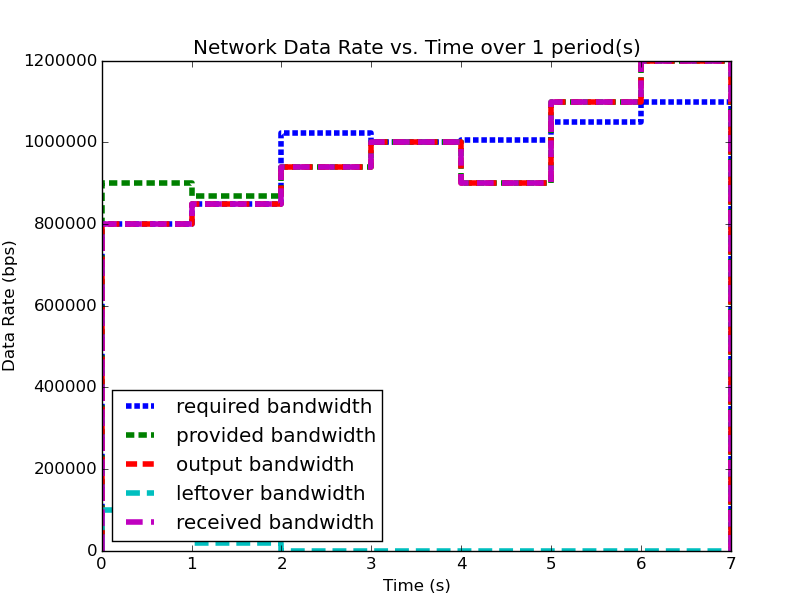
\includegraphics[width=0.8\textwidth]{../doc/src/images/results/1-period-system-bw.png}
  }
  \subfigure[System \emph{(1)} Data for 1 Period]{
    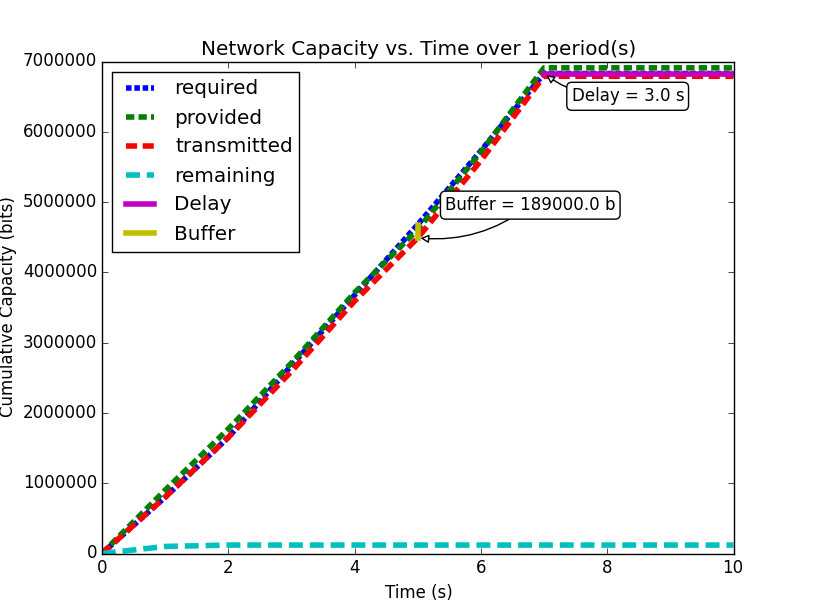
\includegraphics[width=0.8\textwidth]{../doc/src/images/results/1-period-system-data.png}
  }
  \caption{System \emph{(1)} Analyzed over 1 Period}
  \label{fig:1_period_system_1}
\end{figure}

\begin{figure}[ht!]
  \centering
  \subfigure[System \emph{(1)} Data Rate for 2 Periods]{
    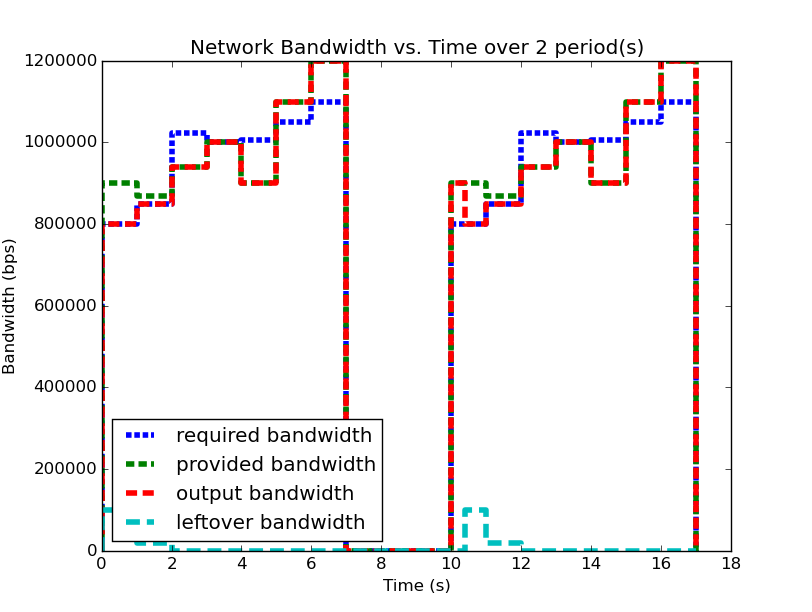
\includegraphics[width=0.8\textwidth]{../doc/src/images/results/2-period-system-bw.png}
  }
  \subfigure[System \emph{(1)} Data for 2 Periods]{
    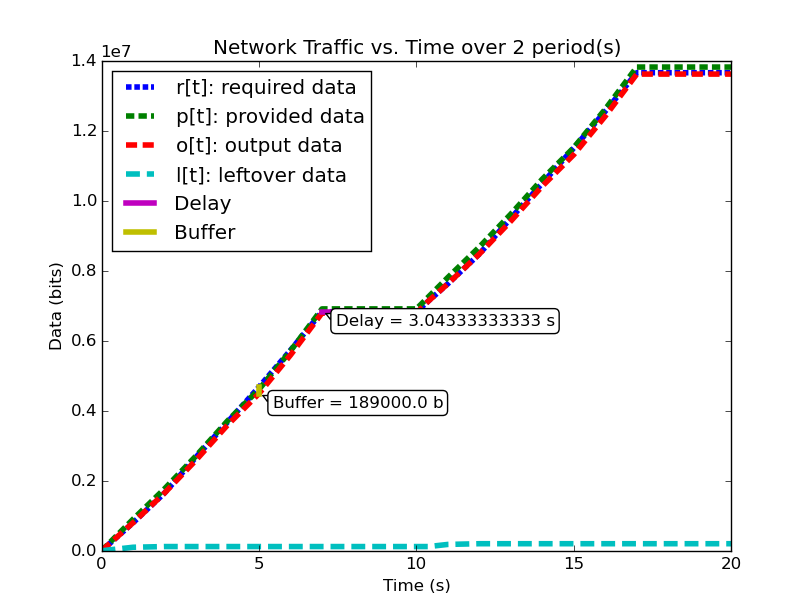
\includegraphics[width=0.8\textwidth]{../doc/src/images/results/2-period-system-data.png}
  }
  \caption{System \emph{(1)} Analyzed over 2 Periods}
  \label{fig:2_period_system_1}
\end{figure}

We notice that for this example system, the second period output
profile is not an exact copy of the first (most easily seen by
examining the bandwidth plots), and yet the required buffer size is
still the same as it was when analyzing the system over one period.
Furthermore, by running the analysis over even larger number of
periods, we can determine (not plotted here for space and
readability), that the predicted buffer size does not change no matter
how many periods we analyze for this system.

Let us look at a system where this is not the case before we begin the
analysis of such system characteristics, shown in
Figure~\ref{fig:1_period_system_2} and Figure~\ref{fig:2_period_system_2}.

\begin{figure}[ht!]
  \centering
  \subfigure[System \emph{(2)} Data Rate for 1 Period]{
    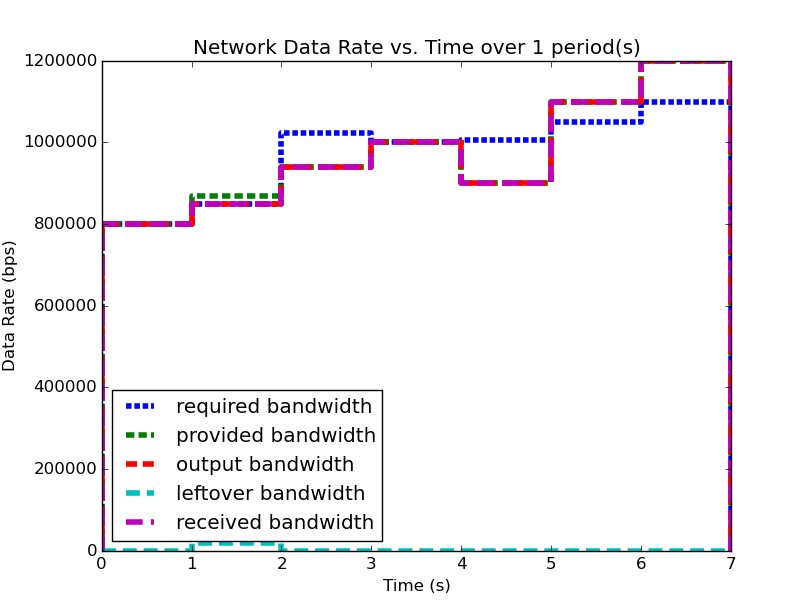
\includegraphics[width=0.8\textwidth]{../doc/src/images/results/1-period-unstable-bw.png}
  }
  \subfigure[System \emph{(2)} Data for 1 Period]{
    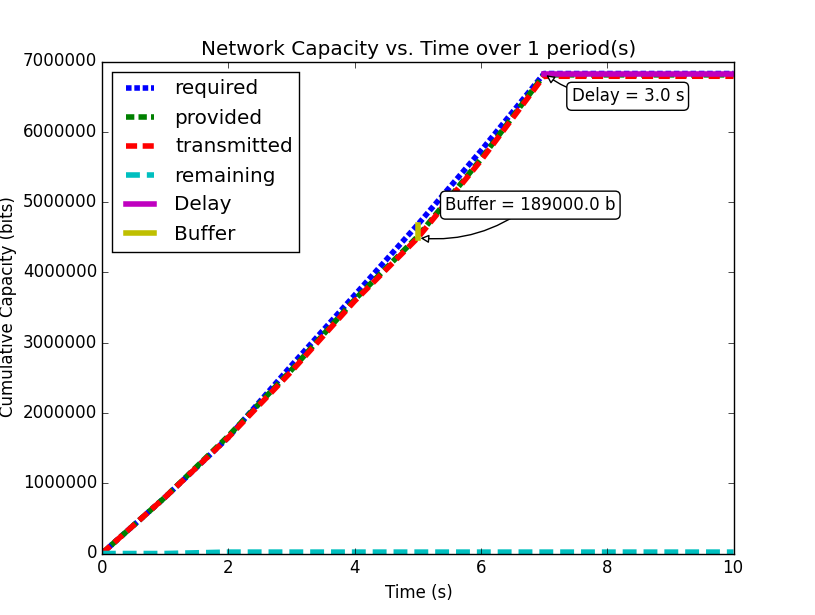
\includegraphics[width=0.8\textwidth]{../doc/src/images/results/1-period-unstable-data.png}
  }
  \caption{System \emph{(2)} Analyzed over 1 Period}
  \label{fig:1_period_system_2}
\end{figure}

\begin{figure}[ht!]
  \centering
  \subfigure[System \emph{(2)} Data Rate for 2 Periods]{
    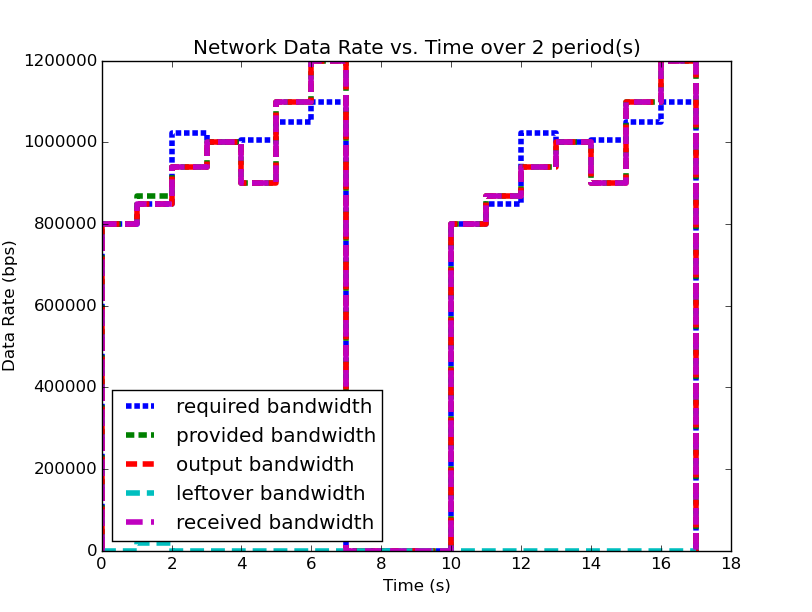
\includegraphics[width=0.8\textwidth]{../doc/src/images/results/2-period-unstable-bw.png}
  }
  \subfigure[System \emph{(2)} Data for 2 Periods]{
    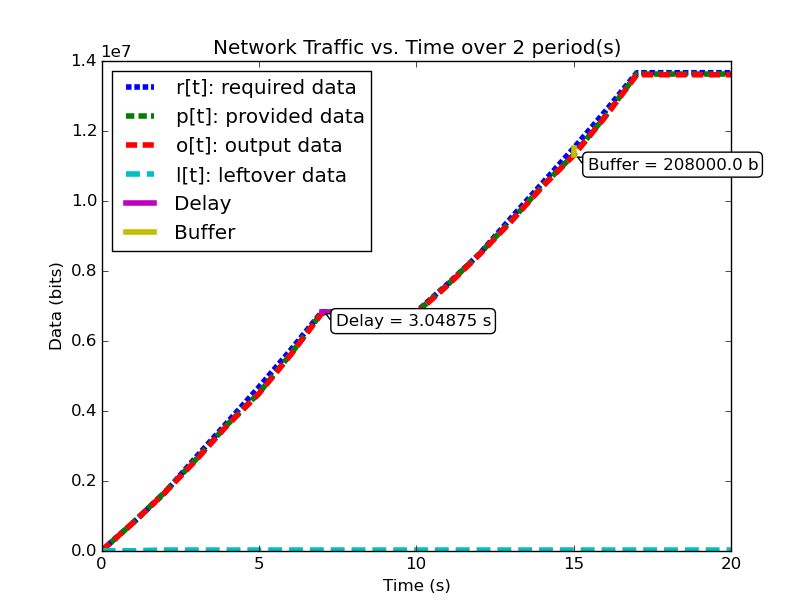
\includegraphics[width=0.8\textwidth]{../doc/src/images/results/2-period-unstable-data.png}
  }
  \caption{System \emph{(2)} Analyzed over 2 Periods}
  \label{fig:2_period_system_2}
\end{figure}

Notice in system \emph{(2)}, the first period analysis predicted the same
buffer size and delay as system \emph{(1)}, but when analyzing two periods
the predicted buffer size changed.  Clearly the behavior of the system
is changing between these two periods.  If we continue to analyze more
periods of system \emph{(2)}, as we did with system \emph{(1)}, we'll find the
unfortunate conclusion that the predicted buffer size increases with
every period we add to the analysis.

We have discovered a system level property that can be calculated from
these profiles, but we must determine what it means and how it can be
used.  First, we see that in system \emph{(1)}, the predicted required
buffer size does not change regardless of the number of periods over
which we analyze the system.  Second, we see that for system \emph{(2)},
the predicted required buffer size changes depending on how many
periods of activity we choose for our analysis window.  Third, we see
that the second period of system \emph{(2)} contains the larger of the two
predicted buffer sizes.  These observations (with our understanding of
deterministic periodic systems) lead us to the conclusion: system
\emph{(2)} can no longer be classified as periodic, since its behavior is
not consistent between its periods.  Furthermore, because the required
buffer size predicted for system system \emph{(2)} continually increases,
we can determine that the system is in fact \emph{unstable} due to
unbounded buffer growth.

\subsection{Proving the Minimum Analysis for System Stability}
\label{subsec:periodic_proof}

Let us now formally prove the assertion about system periodicity and
stability which has been stated above.  We will show that our analysis
results provide quantitative measures about the behavior of the system
and we will determine for how long we must analyze a system to glean
such behaviors.

Typically, periodicity is defined for functions as the equality:

\begin{equation}
  x(t) = x(t + k * T), \forall k \in \mathbb{N} > 0
\end{equation}

but for our type of system analysis this cannot hold since we deal
with cumulative functions (of data vs. time).  Instead we must define
a these functions to be repeating, where a function is repeating
\emph{iff}:

\begin{equation}
  \begin{split}
    x(0) &= 0 \text{  and}\\
    x(t + k * T) &= x(t) + k * x(T), \forall k \in \mathbb{N} > 0
  \end{split}
\end{equation}

Clearly, a repeating function $x$ is \textbf{periodic} \emph{iff}
$x(T)=0$.  Note that repeating functions like the cumulative
data vs. time profiles we deal with, are the result of \textbf{integrating}
\emph{periodic} functions, like the periodic bandwidth vs. time profiles we
use to describe application network traffic and system network
capacity.  All periodic functions, when integrated, produce repeating
functions and similarly, all repeating functions, when differentiated,
produce periodic functions.

Now we will consider a deterministic, \emph{repeating} queuing system
providing a data service function $S$ to input data function
$I$ to produce output data function $O$, where these
functions are \emph{cumulative data versus time}.  At any time $t$,
the amount of data in the system's buffer is given by $B_t$.
After servicing the input, the system has a remaining capacity
function $R$.

\begin{itemize}
\item $S[t]$ : the service function of the system, cumulative data
  service capacity versus time
\item $I[t]$ : the input data to the system, cumulative data versus
  time
\item $O[t]$ : the output data from the system, cumulative data
  versus time
\item $B[t]$ : the amount of data in the system's buffer at time
  $t$, i.e. $I[t]-O[t]$
\item $R[t]$ : the remaining service capacity of the system after
  servicing $I$, i.e. $S[t] - O[t]$
\end{itemize}

Because $S$ and $I$ are deterministic and repeating, they
increase deterministically from period to period, i.e. given the
period $T_I$ of $I$,

\begin{equation}
  \forall t, \forall n \in \mathbb{N} > 0 : I[t + n*T_I] =
  I[t] + n*I[T_I]
\end{equation}

Similarly, given the period $T_S$ of $S$,

\begin{equation}
  \forall t, \forall n \in \mathbb{N} > 0 : S[t + n*T_S] =
  S[t] + n*S[T_S]
\end{equation}

We can determine the hyperperiod of the system as the $lcm$ of
input function period and the service function period, $T_p =
lcm(T_S,T_I)$.

At the start of the system, $t=0$, the system's buffer is empty,
i.e.  $B[0] = 0$.  Therefore, the amount of data in the buffer
at the end of the first period, $t=T_p$, is the amount of data
that entered the system on input function $I$ but was not able
to be serviced by $S$.  At the start of the next period, this
data will exist in the buffer.  Data in the buffer at the start of the
period can be compared to the system's remaining capacity $R$,
since the remaining capacity of the system indicates how much extra
data it can transmit in that period.  Consider the scenario that the
system's remaining capacity $R$ is less than the size of the
buffer, i.e. $R[T_p] < B[T_p]$.  In this scenario,
$B[2*T_p] > B[T_p]$, i.e. there will be more data in the buffer
at the end of the second period than there was at the end of the first
period.  Since the system is deterministic, for any two successive
periods, $n*T_p$ and $(n+1)*T_p$, $B[n*T_p] >
B[(n+1)*T_p]$, which extends to:

\begin{equation}
   B[m*T_p] > B[n*T_p], \forall m>n>0
\end{equation}

implying that:

\begin{equation}
   B[t] < B[t + k*T_p], \forall k \in \mathbb{N} > 0
\end{equation}

meaning that the amount of data in the buffer versus time is \emph{not
periodic}, therefore the amount of data in the system's buffer
increases every period, i.e. the system has \emph{unbounded buffer growth}.

If however, there is enough remaining capacity in the system to
service the data in the buffer, i.e. $R[T_p] >= B[T_p]$, then
$B[2*T_p] = B[T_p]$.  This relation means that if the remaining
capacity of the system that exists after all the period's required
traffic has been serviced is equal to or larger than the size of the
buffer at the end of the period, then in the next period the system
will be able to service fully both the data in the buffer and the
period's required traffic.  Since both the period's traffic and the
buffer's data will have been serviced in that period, the amount of
data in the buffer at the end of the period will be the same as the
amount of data that was in the buffer at the start of the
period. Similarly to above, since the system is deterministic, for any
two successive periods, $n*T_p$ and $(n+1)*T_p$,
$B[(n+1)*T_p] = B[n*T_p]$.  This extends to:

\begin{equation}
   B[m*T_p] = B[n*T_p], \forall m,n > 0
\end{equation}

which implies that:

\begin{equation}
  B[t] = B[t + k*T_p], \forall k \in \mathbb{N} > 0
\end{equation}

meaning that the amount of data in the buffer versus time is a
\emph{periodic function}, therefore the maximum buffer size does not
grow between periods, and the system has a \emph{finite buffer}.

If we are only concerned with buffer growth, we do not need to
calculate $R$, and can instead infer buffer growth by comparing
the values of the buffer at any two period-offset times during the
steady-state operation of the system ($t >= T_p$).  This means
that the system buffer growth check can resolve to $B[2*T_p] ==
B[T_p]$.  This comparison abides by the conditions above, with
$m=2$ and $n=1$.

\newpage
%%%%%%%%%%%%%%%%%%%%%%%%%%%%%%%%%%%%%%%%%%%%%%%%%%%%%%%%%%%%%%%%%%%%%%%%%%%%%%%%%%%
%%%%%%%%%%%%%%%%%%%%%%%%%%%%%%%%%%%%%%%%%%%%%%%%%%%%%%%%%%%%%%%%%%%%%%%%%%%%%%%%%%%
%%%%%%%%%%%%%%%%%%%%%%%%%%%%%%%%%%%%%%%%%%%%%%%%%%%%%%%%%%%%%%%%%%%%%%%%%%%%%%%%%%%
%%%%%%%%%%%%%%%%%%%%%%%%%%%%%%%%%%%%%%%%%%%%%%%%%%%%%%%%%%%%%%%%%%%%%%%%%%%%%%%%%%%
%%%%%%%%%%%%%%%%%%%%%%%%%%%%%%%%%%%%%%%%%%%%%%%%%%%%%%%%%%%%%%%%%%%%%%%%%%%%%%%%%%%

\section{Comparison of \shorttool/ with Network Calculus}
\label{sec:comparison}

When developing a new analysis technique to predict application
network performance, alternative techniques must be evaluated to
determine the utility of the new techniques.  Application developers
and system integrators can then use these comparisons as a metric for
choosing between the available analysis tools.  For the tools and
techniques to affect a meaningful change in system and application
development, they must be shown to be more effective by some metric
for at least certain classes of systems or applications.

To show how our analysis techniques compare to other available
methods, we developed our tools to allow us to analyze the input
system using Network Calculus/Real-Time Calculus techniques as well as
our own.  Using these capabilities, we can directly compare the
analysis results to each other, and then finally compare both results
to the measurements from an actual system.

\subsection{Results}

Figure~\ref{fig:system_comparison} shows the data rate versus time
profile describing the example system, side-by-side with the
time-integrated and analyzed data versus time profile.
Figure~\ref{fig:zoom_pnp} shows a zoomed in portion of the second
plot, focusing on the area with the maximum delay and buffer as
analyzed by \shorttool/.  Figure~\ref{fig:nc_comparison} shows the
same system analyzed using Network Calculus.

\begin{figure}[ht!]
  \centering
  \subfigure[System Data Rate vs. Time]{
    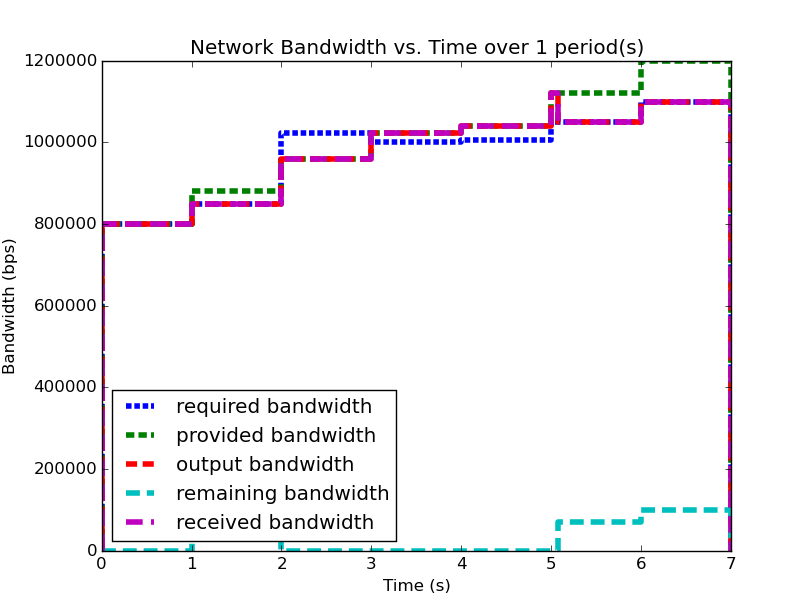
\includegraphics[width=0.8\textwidth]{../doc/src/images/results/maren_namek_bw.png}
  }
  \subfigure[System Data Analyzed with \shorttool/]{
    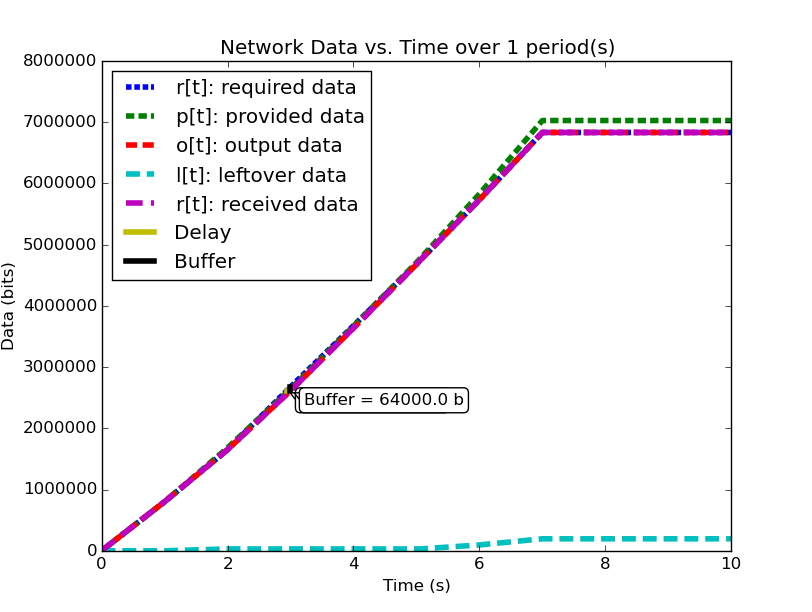
\includegraphics[width=0.8\textwidth]{../doc/src/images/results/maren_namek_data.png}
    \label{subfig:pnp_analysis_comparison}
  }
  \caption{System profile used for comparison of \shorttool/ with
    Network Calculus.  The Analysis using \shorttool/ is shown on the right.}
  \label{fig:system_comparison}
\end{figure}

\begin{figure}[ht!]
  \centering
  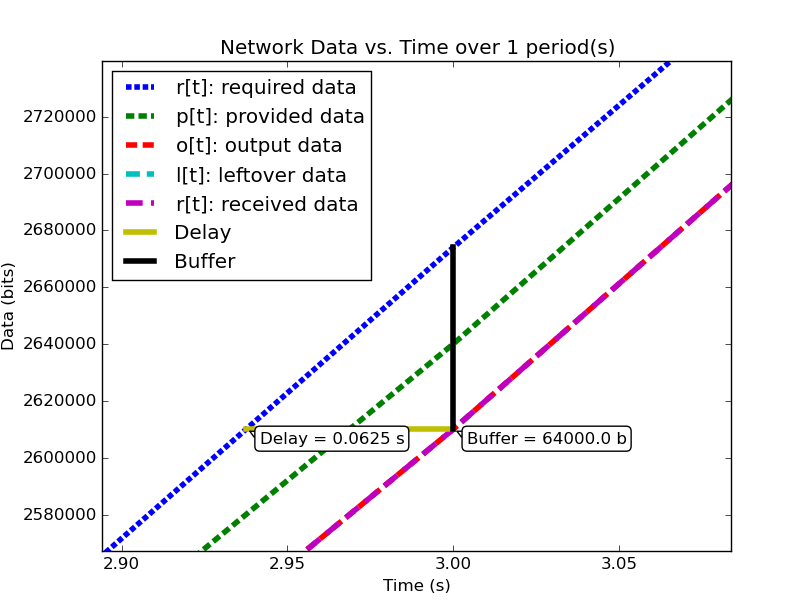
\includegraphics[width=0.85\textwidth]{../doc/src/images/results/maren_namek_data_zoom.png}
  \caption{Zoomed-in version of
    Figure~\ref{subfig:pnp_analysis_comparison}, focusing on the
    predicted buffer and delay.}
  \label{fig:zoom_pnp}
\end{figure}

\begin{figure}[ht!]
  \centering
  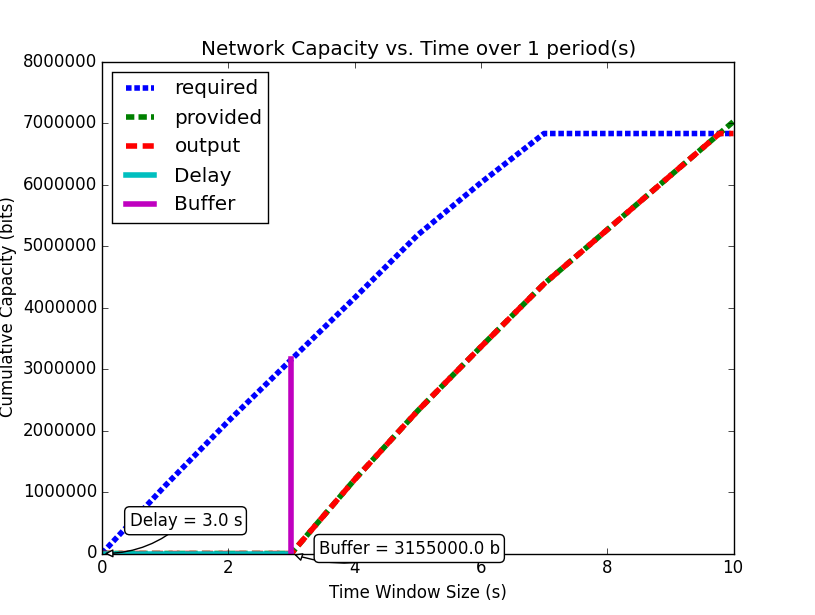
\includegraphics[width=0.85\textwidth]{../doc/src/images/results/nc_namek_data.png}
  \caption{Network-Calculus based analysis of the same system.}
  \label{fig:nc_comparison}
\end{figure}

The major drawback for Network Calculus that our work aims to solve is
the disconnect from the real system that stems from using an approach
based on time-window analysis.  Such an approach leads to dramatically
under-approximating the capacity of the network while simultaneously
over-approximating the utilization of the network, since a known drop
in network performance which is expected and handled by the
application cannot be accurately modeled.  In our case, the system is
using a system profile which can service data during the period from
$0\le t\le 7$ seconds with a period of 10 seconds.  The
application is designed around this constraint and only produces data
during that interval.  Because our technique directly compares when
the application produces data to when the system can service the data,
we are able to derive more precise performance prediction metrics than
Network Calculus, which compares the 3 seconds of system downtime to
the 3 seconds of maximum application data production.

%We developed software which produces data according to a supplied
%input profile and configured the system's network to provide the
%bandwidth profile described in the system configuration profile.

Using the same testbed, traffic production software, and traffic
measurement software described in Section~\ref{subsec:precision}, we
were able to measure the transmitted traffic profile, the received
traffic profile, the latency experienced by the data, and the
transmitter's buffer requirements.  The results are displayed in
Table~\ref{table:results} (from the same experimental data as in
Section~\ref{subsec:precision}):

\begin{table}[htbp]
\caption{Experimental system measurements}
\begin{tabular}{| c | c | c | c |}
\hline
 & Network Calculus & $PNP^2$ & Measured ($\mu,\sigma$) \\\hline
Buffer Delay (s) & 3.0 & 0.0625 & (0.06003 , 0.00029) \\\hline
Time of Delay (s) & N/A & 3.0 & (2.90547 , 0.00025) \\\hline
Buffer Size (bits) & 3155000 & 64000 & (61780.72 , 295.52) \\\hline
\end{tabular}
\label{table:results}
\end{table}

Taking the results from our published work, where our methods
predicted a buffer size of 64000 bits, we show that Network Calculus
predicts a required buffer size of 3155000 bits. This drastic
difference comes from the mis-match between down-time and max data
production mentioned above.  Note also that Network Calculus does not
provide a way to predict when (during the run-time of the
applications) the maximum delay will occur.  Network Calculus lacks
this capability because it defines its models as functions of
time-window size instead of as direct functions of time.

\newpage
%%%%%%%%%%%%%%%%%%%%%%%%%%%%%%%%%%%%%%%%%%%%%%%%%%%%%%%%%%%%%%%%%%%%%%%%%%%%%%%%%%%
%%%%%%%%%%%%%%%%%%%%%%%%%%%%%%%%%%%%%%%%%%%%%%%%%%%%%%%%%%%%%%%%%%%%%%%%%%%%%%%%%%%
%%%%%%%%%%%%%%%%%%%%%%%%%%%%%%%%%%%%%%%%%%%%%%%%%%%%%%%%%%%%%%%%%%%%%%%%%%%%%%%%%%%
%%%%%%%%%%%%%%%%%%%%%%%%%%%%%%%%%%%%%%%%%%%%%%%%%%%%%%%%%%%%%%%%%%%%%%%%%%%%%%%%%%%
%%%%%%%%%%%%%%%%%%%%%%%%%%%%%%%%%%%%%%%%%%%%%%%%%%%%%%%%%%%%%%%%%%%%%%%%%%%%%%%%%%%

\section{Analysis of TDMA Scheduling}
\label{sec:tdma}

Medium channel access protocols are used in networking systems to
govern the communication between computing nodes which share a network
communications medium.  They are designed to allow reliable
communication between the nodes, while maintaining certain goals, such
as minimizing network collisions, maximizing bandwidth, or maximizing
the number of nodes the network can handle.  Such protocols include
Time Division Multiple Access (TDMA), which tries to minimize the
number of packet collisions; Frequency Division Multiple Access
(FDMA), which tries to maximize the bandwidth available to each
transmitter; and Code Division Multiple Access (CDMA) which tries to
maximize the number of nodes that the network can
handle\cite{jung1993advantagesCDMAFDMATDMA}.  We will not discuss CDMA
in the scope of this work.

In FDMA, each node of the network is assigned a different transmission
frequency from a prescribed frequency band allocated for system
communications.  Since each node transmits on its own frequency,
collisions between nodes transmitting simultaneously are reduced.
Communications paradigms of this type, i.e. shared medium with
collision-free simultaneous transmission between nodes, can be modeled
easily by our \shorttool/ modeling paradigm described above, since the
network resource model for each node can be developed without taking
into account the transmissions of other nodes.

In TDMA, each node on the network is assigned one or more time-slots
per communications period in which only that node is allowed to
transmit.  By governing these timeslots and having each node agree
upon the slot allocation and communications period, the protocol
ensures that at a given time, only a single node will be transmitting
data, minimizing the number of collisions due to multiple simultaneous
transmitters.  In such a medium access protocol, transmissions of each
node affect other nodes' transmission capability.  Because these
transmissions are scheduled by TDMA, they can be explicitly integrated
into the system network resource model.

\subsection{Problem}
TDMA transmission scheduling has an impact on the timing
characteristics of the applications' network communications.  Because
applications' network data production is decoupled from their node's
TDMA transmission time slot, buffering may be required when an
application on one node tries to send data on the network during the
transmission slot of a different node.  In this case, the data would
need to be buffered on the application's node and would therefore
incur additional buffering delay.  If this TDMA schedule is not
integrated into the analysis of the network resources, the additional
buffer space required may exceed the buffer space allocation given to
the application or the buffering delay may exceed the application's
acceptable latency.

\subsection{Results}

So far, the description of the system provided network service profile
($p[t]=y$), has been abstracted as simply the available
bandwidth as a function of time integrated to produce the amount of
data serviced as a function of time. We show how to model and analyze
the network's lower-level TDMA MAC protocol using our network modeling
semantics.  We then derive general formulas for determining the affect
TDMA has on buffer size and delay predictions.

As an example TDMA system which benefits from our analysis techniques,
consider an application platform provided by a fractionated satellite
cluster.  For this system, the network between these satellites is a
precious resource shared between each of the applications' components
in the cluster.  To ensure the stability of the network resources,
each satellite has a direct connection to every other satellite and is
assigned a slot in the TDMA schedule during which the satellite may
transmit.  Each TDMA slot has a sinusoidally time-varying bandwidth
profile which may differ from the other TDMA slot bandwidth profiles.
The time-varying profile of the slot bandwidth comes from the coupling
between the radios' inverse-squared
bandwidth-as-a-function-of-distance and the satellites' sinusoidal
distance-as-a-function-of-orbital-position, as described in
Section~\ref{sec:intro}. The requirement for accurate performance
prediction necessitates the incorporation of the TDMA schedule into
the network modeling and analysis.

TDMA schedules can be described by their period, their number of
slots, and the bandwidth available to each slot as a function of time.
For simplicity of explanation, we assume that each node only gets a
single slot in the TDMA period and all slots have the same length, but
the results are valid for all static TDMA schedules.  Note that each
slot still has a bandwidth profile which varies as a function of time
and that each slots may have a different bandwidth profile.

In a given TDMA period $T$, a node $n$ can transmit a certain number
of bits governed by its slot length $t_{n}$ and the slot's available
bandwidth $bw_{n}$.  During the rest of the TDMA period, the node's
available bandwidth is $0$.  This scheduling has the effect of
amortizing the node's slot bandwidth into an effective bandwidth of
$bw_{effective}$.  The addition of the TDMA scheduling can affect the
buffer and delay calculations, based on the slot's bandwidth, the
number of slots, and the slot length.  The maximum additional delay is
$\Delta_{delay}$, and the maximum additional buffer space is
$\Delta_{buffer}$.  These deviations are shown graphically by
Figure~\ref{fig:tdma} and calculated by
\begin{equation}
  \begin{split}
    bw_{effective} &= bw_{n} * \dfrac{t_n}{T}\\
    \Delta_{delay} &= T - t_{n}\\
    \Delta_{buffer} &= \Delta_{delay} * bw_{effective}
  \end{split}
  \label{eq:tdma}
\end{equation}
Where:
\begin{itemize}
\item $T$ is the period of the TDMA schedule
\item $t_n$ is the length of node $n$'s TDMA slot
\item $bw_n$ is the bandwidth available to node $n$ during its slot
\item $bw_{effective}$ is the perceived bandwidth available to the
  node during the TDMA period
\item $\Delta_{delay}$ is the change in the predicted delay
  experienced by application traffic on the network
\item $\Delta_{buffer}$ is the change in the predicted buffer space
  required for lossless transmission of application traffic
\end{itemize}
Clearly, $\Delta_{delay}$ is bounded by $T$
and $\Delta_{buffer}$ is governed by $t_{n}$.  Therefore, because
$t_{n}$ is dependent on $T$, minimizing $T$ minimizes both the maximum
extra delay and maximum extra buffer space.
\begin{figure}[ht!]
  \centering
  \subfigure[In-Phase TDMA Profile vs Abstract]{
    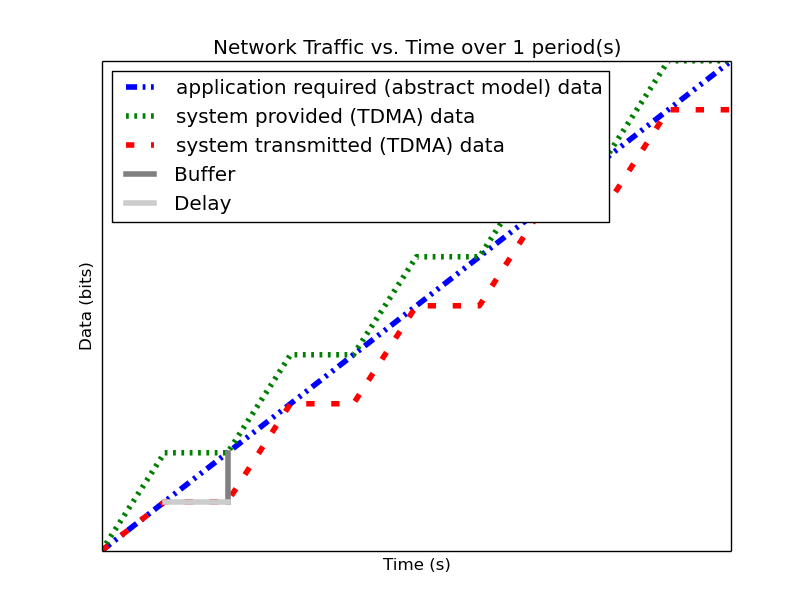
\includegraphics[width=0.8\textwidth]{../doc/src/images/results/tdma_phase0.png}
  }
  \subfigure[Out-of-Phase TDMA Profile vs Abstract]{
    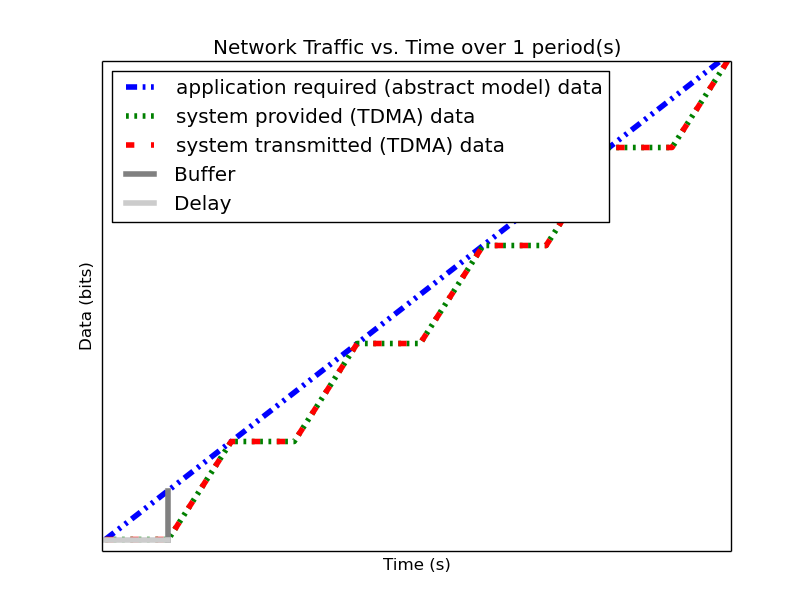
\includegraphics[width=0.8\textwidth]{../doc/src/images/results/tdma_phase1.png}
  }
  \caption{Effects of TDMA scheduling in the MAC layer on system
    network performance.}
  \label{fig:tdma}
\end{figure}

Following from this analysis, we see that if: (1) the TDMA effective
bandwidth profile is provided as the abstract system network service
profile, and (2) the TDMA period is much smaller than the duration of
the shortest profile interval; then the system with explicit modeling
of the TDMA schedule has similar predicted application network
characteristics as the abstract system.  Additionally, the maximum
deviation formulas derived above provide a means for application
developers to analyze the their application on a TDMA system without
explicitly integrating the TDMA model into the system profile model.

Through the analysis of TDMA scheduling's effect on application level
performance prediction, we derived analytical formulas for the maximum
deviation between the abstract system model and the model with
explicitly encoded TDMA scheduling.  The use of these formulas frees
developers and system integrators from having to explicitly
incorporate the TDMA schedule in their application and system models.
This TDMA modeling and analysis was published in
\cite{ISIS_F6_ISORC_QOS:15}.

\newpage
%%%%%%%%%%%%%%%%%%%%%%%%%%%%%%%%%%%%%%%%%%%%%%%%%%%%%%%%%%%%%%%%%%%%%%%%%%%%%%%%%%%
%%%%%%%%%%%%%%%%%%%%%%%%%%%%%%%%%%%%%%%%%%%%%%%%%%%%%%%%%%%%%%%%%%%%%%%%%%%%%%%%%%%
%%%%%%%%%%%%%%%%%%%%%%%%%%%%%%%%%%%%%%%%%%%%%%%%%%%%%%%%%%%%%%%%%%%%%%%%%%%%%%%%%%%
%%%%%%%%%%%%%%%%%%%%%%%%%%%%%%%%%%%%%%%%%%%%%%%%%%%%%%%%%%%%%%%%%%%%%%%%%%%%%%%%%%%
%%%%%%%%%%%%%%%%%%%%%%%%%%%%%%%%%%%%%%%%%%%%%%%%%%%%%%%%%%%%%%%%%%%%%%%%%%%%%%%%%%%

\section{Compositional Analysis}
\label{sec:compositional_analysis}

Now that we have precise network performance analysis for aggregate
profiles or singular profiles on individual nodes of the network, we
must determine how best to compose these profiles and nodes together
to analyze the overall system.  The aim of this work is to allow the
profiles from each application to be analyzed separately from the
other profiles in the network, so that application developers and
system integrators can derive meaningful performance predictions for
specific applications.  For this goal, let us define:

\begin{definition}[Compositionality]\cite{sifakis2002}
  A system is compositional if its properties can be derived from
  the properties of its components and how they are interconnected.
\end{definition}

\begin{definition}[Composability]\cite{sifakis2002}
  A component is composable if its properties do not change
  when the component is composed with other components.
\end{definition}

For our analysis techniques to be compositional, an application's
required profile must be analyzable individually without requiring
aggregation with the rest of the required profiles in the system.
This means that the system's performance, i.e. the performance of all
the applications on the system, can be determined by analyzing the
performance of each application individually.

To achieve compositionality, we must not only define mathematical
operations which allow us to aggregate and separate profiles with/from
each other, but also the semantics of how these profiles are composed
with one another.  This semantics govern the relation between
required profiles, specifically governing the distribution of their
shared node's provided profile between each other.  For our
compositional analysis, we defined that each required profile in the
system be given a unique priority, $U$, with the relation that a
profile $P_1$ has a higher priority than profile $P_2$
\emph{iff} $U_{P_1} < U_{P_2}$.  Using this priority relation, we can
define that a profile $P_i$ does not receive any capacity from
its node at time $t$ until all other profiles with priority
$< U_{P_i}$ have received their requested capacity from the
node at $t$.  If the node does not have enough capacity at
$t$ to service $P_i$, then the data $P_i$ attempted
to send at $t$ will be placed into its buffer, to be sent at a
time when the node has available bandwidth for $P_i$.

This priority relation for compositional analysis is similar to the
task priority used for schedulability analysis in Real-Time Calculus,
mentioned in :ref:$rtc$.  Similarly to RTC, this priority relation and
compositionality allow us to capture the effects independent profiles
have on each other when they share the same network resources.  Just
as RTC based its priority relation and computation scheduling on a
fixed-priority scheduler, our priority relation and resource allotment
is based on the network Quality-of-Service (QoS) management provided
by different types of networking infrastructure.  One such mechanism
for implementing this type of priority-based network resource
allocation is through the use of the DiffServ Code Point
(DSCP)\cite{rfc2474}.  The DSCP is a bit-field in all packets which
have an Internet Protocol (IP) header which allows the packet to be
assigned a specific class for per-hop routing behavior.  Routers and
forwarders in the network group packets according to their DSCP class
and provide different service capacities to each class.  For example,
the \emph{Expedited Forwarding} \cite{rfc3246} class receives strict
priority queuing above all other traffic, which makes it a suitable
implementation of this type of resource allocation.  Similarly, the
Linux Traffic Control\cite{linux_tc} utility provides many mechanisms
for shaping, policing, routing, and classifying traffic.  Its
class-based queuing disciplines and filtering mechanisms provide the
capability for such strict priority-based network resource
allocation.  

Mathematically, compositionality requires that we be able to add and
subtract profiles from each other, for instance to determine the
remaining service capacity of a node available for a profile $P_i$
after it serves all profiles with a higher priority.  Queuing of the
lower priority profiles is taken into account when the lower priority
profile is convolved with the remaining capacity the node has
available to service it.  The calculation of the remaining capacity,
$P_P'$, of the node after it services $P_i$ is given as:
\begin{equation}
  P_P' = P_P - ( P_i \otimes P_P )
\end{equation}
Where
\begin{itemize}
\item $P_P$ is the capacity available to profile $P_i$
\end{itemize}

Mathematically, addition and subtraction of two profiles $f[t],g[t]$ are given by:
\begin{equation}
  s[t] = f[t] + g[t]
\end{equation}
and
\begin{equation}
  s[t] = f[t] - g[t]
\end{equation}

Experimental validation of these compositional techniques,
specifically with respect to priority relation, adding, and
subtracting of profiles is presented at the end of
Section~\ref{sec:routing}.

\newpage
%%%%%%%%%%%%%%%%%%%%%%%%%%%%%%%%%%%%%%%%%%%%%%%%%%%%%%%%%%%%%%%%%%%%%%%%%%%%%%%%%%%
%%%%%%%%%%%%%%%%%%%%%%%%%%%%%%%%%%%%%%%%%%%%%%%%%%%%%%%%%%%%%%%%%%%%%%%%%%%%%%%%%%%
%%%%%%%%%%%%%%%%%%%%%%%%%%%%%%%%%%%%%%%%%%%%%%%%%%%%%%%%%%%%%%%%%%%%%%%%%%%%%%%%%%%
%%%%%%%%%%%%%%%%%%%%%%%%%%%%%%%%%%%%%%%%%%%%%%%%%%%%%%%%%%%%%%%%%%%%%%%%%%%%%%%%%%%
%%%%%%%%%%%%%%%%%%%%%%%%%%%%%%%%%%%%%%%%%%%%%%%%%%%%%%%%%%%%%%%%%%%%%%%%%%%%%%%%%%%

\section{Delay Analysis}
\label{sec:delay}

When dealing with queuing systems (esp. networks) where precise
design-time guarantees are required, the delay in the links of the
network must be taken into account.

The delay is modeled as a continuous function of latency (seconds)
versus time.  In the profiles, the latency is specified discretely as
$(time, latency)$ pairs, and is interpolated linearly between
successive pairs.  Specifically, $time$ is a time point at which the
latency on the link is given by $latency$.  

Using this latency semantics, the delay convolution of a profile
becomes

\begin{equation}
  r[t + \delta[t]] = l[t]
\end{equation}

Where

\begin{itemize}
\item $l[t]$ is the \emph{link} profile describing the data as a
  function of time as it enters the link
\item $\delta[t]$ is the \emph{delay} profile describing the latency
  as a function of time on the link
\item $r[t]$ is the \emph{received} profile describing the data as a
  function of time as it is received at the end of the link
\end{itemize}
  
When analyzing delay in a periodic system, it is important to
determine the effects of delay on the system's periodicity.  We know
that the period of the periodic profiles is defined by the time
difference between the start of the profile and the end of the
profile.  Therefore, we can show that if the time difference between
the \textbf{start time} of the \emph{received} profile and the
\textbf{end time} of the \emph{received} profile is the same as the
\textbf{period} of the \emph{link} profile, the periodicity of the
profile is unchanged.

\begin{itemize}
\item $T_p$ is the period of the \emph{link} profile
\item $r[t + \delta[t]]$ is the beginning of the \emph{received}
  profile
\item $r[(t + T_p) + \delta[(t + T_p)]]$ is the end of the
  \emph{received} profile
\end{itemize}

We determine the condition for which $(t_{end}) - (t_{start}) =
T_p$:

\begin{equation}
  \begin{split}
    (T_p + t + \delta[T_p + t]) - (t + \delta[t]) &= T_p \\
    T_p + \delta[T_p + t] - \delta[t] &= T_p \\
    \delta[T_p + t] - \delta[t] &= 0\\
    \delta[T_p + t] &= \delta[t]
  \end{split}
\end{equation}

Which is just confirms that the periodicity of the delayed profile is
unchanged \emph{iff} the latency profile is \textbf{periodic}, i.e.

\begin{equation}
\delta[t] = \delta[t + k*T_p], \forall k\in\mathbb{N} > 0
\end{equation}

Experimental validation of this delay analysis is presented at the end
of Section~\ref{sec:routing}.

\newpage
%%%%%%%%%%%%%%%%%%%%%%%%%%%%%%%%%%%%%%%%%%%%%%%%%%%%%%%%%%%%%%%%%%%%%%%%%%%%%%%%%%%
%%%%%%%%%%%%%%%%%%%%%%%%%%%%%%%%%%%%%%%%%%%%%%%%%%%%%%%%%%%%%%%%%%%%%%%%%%%%%%%%%%%
%%%%%%%%%%%%%%%%%%%%%%%%%%%%%%%%%%%%%%%%%%%%%%%%%%%%%%%%%%%%%%%%%%%%%%%%%%%%%%%%%%%
%%%%%%%%%%%%%%%%%%%%%%%%%%%%%%%%%%%%%%%%%%%%%%%%%%%%%%%%%%%%%%%%%%%%%%%%%%%%%%%%%%%
%%%%%%%%%%%%%%%%%%%%%%%%%%%%%%%%%%%%%%%%%%%%%%%%%%%%%%%%%%%%%%%%%%%%%%%%%%%%%%%%%%%

\section{Analysis of Statically Routed Networks}
\label{sec:routing}

\subsection{Problem}
As CPS become more distributed in nature and begin to act as
infrastructure for distributed applications towards IoT systems, they
will necessarily need to handle more network resource management and
network connection routing within their network as well as between
their own network and any external networks to which they are
connected.  Such networks generally rely on routing to allow more
flexibility in the system with respect to node placement and
connectivity.  Adding routing to the network also has the effect of
increasing the complexity of the network performance analysis and can
cause drastic differences in application network performance when
compared with networks without routing.  Therefore the design-time
analysis tools which help predict application network performance must
take this routing into account.  It should be noted that this is a
special case of routing in ad-hoc networks, where one or more nodes
can route messages for other nodes.

\subsection{Results}
Having discussed profile composition and the affects of delaying a
profile, we can address one more aspect of system analysis:
\emph{routing}.  For this analysis we will specifically focus on
statically routed networks.

Firstly, we must define the assumptions we make about the router nodes
with respect to how they forward the network traffic.  In our modeling
and analysis, because we have not considered transmission
error/corruption, we are most closely modeling cut-through routing /
wormhole switching in which the routing and forwarding nodes in the
system forward all packets without checking them for corruption or
integrity.  This forwarding mechanism differs from store and forward
routing in which each packet is checked for errors in its entirety
before sending it to the next node on its route.  In the case of store
and forward, when a corrupt packet is received by a routing node, it
will not forward that packet along its path, and may optionally
request re-transmission of the packet from the previous node.  Under
the assumption of no transmission errors, we can incorporate the added
latency incurred by store and forward into the latency profile of the
router node.  In this way, these two forwarding techniques can be
modeling in a simple way using our semantics (where they both simply
affect the latency of the node).  

Given these assumptions about the forwarding techniques of the routing
nodes, we can describe system-level analysis.  By incorporating both
the latency analysis with the compositional operations we developed,
we can perform system-level analysis of profiles which are routed by
nodes of the system.  In this paradigm, nodes can transmit/receive
their own data, i.e. they can host applications which act as data
sources or sinks, as well as act as routers for profiles from and to
other nodes.  To make such a system amenable to analysis we must
ensure that we know the routes the profiles will take at design time,
i.e. the routes in the network are static and known or calculable.
Furthermore, we must, for the sake of profile composition as described
above, ensure that each profile has a priority that is unique within
the network which governs how the transmitting and routing nodes
handle the profile's data.

Let us define the system configuration $C$ as:

\begin{equation}
  C = \{\{P_S\},\{N\},\{R\}\}
\end{equation}

Where

\begin{itemize}
\item $\{P_S\}$ is the \emph{set} of all \emph{sender} profiles in the system
  configuration
\item $\{N\}$ is the \emph{set} of all \emph{nodes} in the system configuration, and
\item $\{R\}$ is the \emph{set} of all \emph{routes} in the system configuration
\end{itemize}

We define a profile $P$ as:

\begin{equation}
  P = \{N_I,K,T,F,U,\{(t,R_D,D,L)\}\}
\end{equation}

Where

\begin{itemize}
\item $N_I$ is the \emph{Node ID} to which the profile applies
\item $K$ is the \emph{kind} of the profile, where
  $K\in\{provided,required,receiver\}$
\item $T$ is the \emph{period} of the profile
\item $F$ is the \emph{flow ID} of the profile, where two profiles,
  $P_1,P_2$ belong to the same flow \emph{iff}
  $F_{P_1}==F_{P_2}$
\item $U$ is the \emph{priority} of the profile, where profile
  $P_1$ has a higher priority than profile $P_2$ \emph{iff}
  $U_{P_1} < U_{P_2}$, and
\item $\{(t,R_D,D,L)\}$ is a \emph{set} of $(time, data\ rate,
  data, latency)$ tuples describing how each of $\{data\ rate,
  data, latency\}$ vary with respect to time.  Semantically, the
  $data\ rate$ is constant between any two successive values of
  $t$, while the $data$ and $latency$ are \emph{linearly
  interpolated} during the same interval.  The initial profile
  specification does not have the $data$ field; $data$ is
  calculated based on $data\ rate$.
\end{itemize}

Then we define a node $N$ as:

\begin{equation}
  N = \{I,P_P,\{P_R\}\}
\end{equation}

Where 

\begin{itemize}
\item $I$ is the \emph{ID} of the node
\item $P_P$ is the \emph{provided} profile of the node, and
\item $\{P_R\}$ is the \emph{set} of all \emph{receiver} profiles on the node
\end{itemize}

And finally, we define a route $R$ as:

\begin{equation}
  R = \{N_{I_1},N_{I_2},...,N_{I_N}\}
\end{equation}

Where

\begin{equation}
  \forall N_X,N_Y \subset N, \exists! R_{X,Y} = \{N_{I_X},...,N_{I_Y}\}
\end{equation}

We can then run Algorithm~\ref{lst:routing_alg} to iteratively analyze
the system.  In this algorithm, the remaining capacity of the node is
provided to each profile with a lower priority iteratively.  Because
of this iterative recalculation of node provided profiles based on
routed profiles, we directly take into account the effect of multiple
independent profiles traversing the same router; the highest priority
profile receives as much bandwidth as the router can give it, the next
highest priority profile receives the remaining bandwidth, and so on.

\begin{listing}[ht!]
  \begin{minted}{python}
  analyze( sender_profiles )
  {
    sender_profiles = sorted(sender_profiles, priority)
    for required_profile in sender_profiles
    {
      transmitted_nodes = list.empty() 
      for receiver_profile in
          required_profile.receiver_profiles()
      {
        route =
          getRoute(required_profile, receiver_profile)
        for node in route
        {
          if node in transmitted_nodes
            and multicast == true
	  {
	    continue
	  }
	  provided_profile = node.provided_profile
            
	  output_profile =
            convolve(required_profile, provided_profile)
	  remaining_profile =
            provided_profile - output_profile
	  received_profile =
            delay(output_profile, provided_profile)
            
	  node.provided_profile = remaining_profile
	  required_profile = received_profile
	  transmitted_nodes.append(node)
        }
        receiver_received_profile =
          convolve(required_profile, receiver_profile)
      }
    }
  }
  \end{minted}
  \caption{Algorithm for iteratively analyzing profiles in a
    distributed system with static routing and profile priorities.}
  \label{lst:routing_alg}
\end{listing}

We take care of matching all senders to their respective receivers,
and ensure that if the system supports multicast, a no re-transmissions
occur; only nodes which must route the profile to a new part of the
network re-transmit the data.  However, if the system does not support
multicast, then the sender must issue a separate transmission, further
consuming network resources.  In this way, lower-level transport
capabilities can be at least partially accounted for by our analysis.

We have implemented these functions for statically routed network
analysis into our tool, which automatically parses the profiles, the
network configuration and uses the algorithm and the implemented
mathematics to iteratively analyze the network.  Analytical results
for example systems will be provided when the experimental results can
be used as a comparison.

To determine the validity of our routing, composition, and delay
analysis, we developed a sample system and application deployment
consisting of two flows generated by two profiles, one a high priority
flow and one a low priority flow.  Each flow originates on a separate
computing node, with different destinations.  Both flows are routed
through the same routing node that enforces priority-based routing for
the two flows.  Figure~\ref{fig:routing_example} shows the
configuration of the system and application for the experimental
validation of the routing, composition, and delay analysis techniques.

\begin{figure}[ht!]
  \centering
  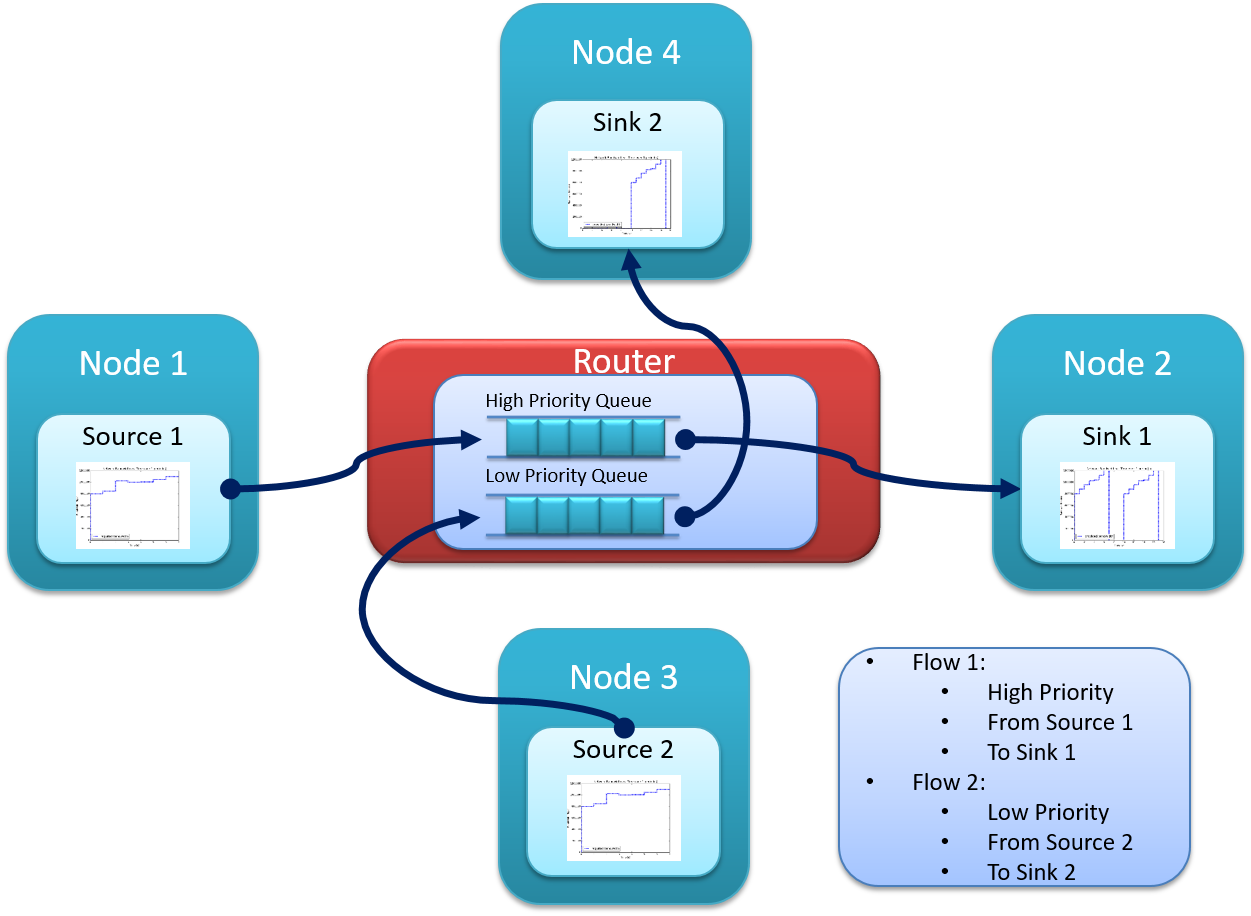
\includegraphics[width=\textwidth]{./figs/routing_example.png}
  \caption{Experimental setup to validate routing, delay, and
    compositional analysis of network profiles.}
  \label{fig:routing_example}
\end{figure}

For this experimental setup, we configured the Linux kernel using
TC\cite{linux_tc} which provides mechanisms for implementing traffic
prioritization, shaping, and delay, among other features. All
application traffic on each node passed through shaping and delay
queues, which shaped the application traffic according to the
properties of its system profile.  Additionally, for the router node
we configured priority queuing which filtered the application traffic
into a high priority queue and a low priority queue.  These queues are
dequeued in the kernel according to priority FIFO, which means that
data will not be dequeued from lower priority queues unless all high
priority queues are empty.  These priority queues feed into traffic
shaper and delay queues, to enforce the system profile on the
traffic.  This configuration is shown schematically in
Figure~\ref{fig:network_traffic}.  A more detailed description of the
specific configuration and operation of TC is given in
Appendix~\ref{ch:tc}.

\begin{figure}[ht!]
  \centering
  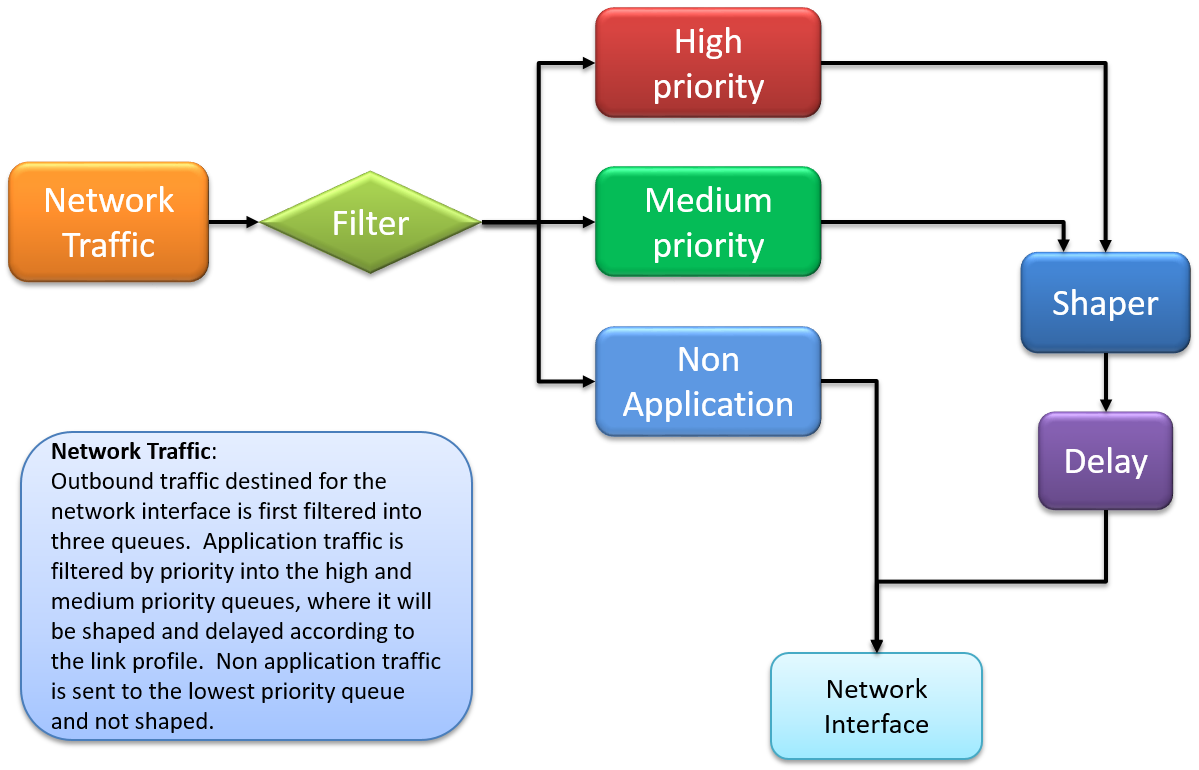
\includegraphics[width=\textwidth]{./figs/network_traffic.png}
  \caption{Diagram illustrating the flow of network traffic through
    the priority queues and traffic shaping in the kernel.}
  \label{fig:network_traffic}
\end{figure}

This experimental setup allows us to examine the validity of our
analysis techniques in the following ways:

\begin{itemize}
  \item Because the system implements the strict priority queuing of
    flows, especially independent interacting flows, we can compare
    the delay and buffering measurements to the same delay and buffer
    predictions from the model.
  \item Router buffer space requirements can be measured and compared
    with their predicted requirements to validate routed network
    analysis.
  \item Link delay composition can be validated by examining the
    receiver buffer requirements compared with the predicted receiver
    buffer sizes.  
\end{itemize}

\iffalse
Using this system and application configuration, we can validate the
analysis results by comparing:

\begin{itemize}
  \item The delay measured between the reception of data and
    transmission of data \emph{versus} the predicted delay
  \item The buffer measured between on the receiver end of the data
    flow \emph{versus} the predicted receiver buffer size for each flow
\end{itemize}

Additionally, the analysis techniques are useful for predicting the
required buffer size on the routing node for each of the queues
corresponding to the two flows.  Because we can directly control the
size of these queues, we can show that if we configure their sizes to
be the analysis' predicted sizes and we lose no messages then the
predicted buffer sizes are sufficient for the system and application
configuration.  
\fi

The results of our experiments using this application and system
configuration are shown in Table~\ref{table:routing_results}.
Similarly to our earlier experimental results, the predictions of the
overall delay for both the high and low priority routed flows are
conservative, but tight bounds on the actual delay experienced by the
flows in the routed network with delays.

\begin{table}[htbp]
\caption{Delay and Buffer Results: Prediction versus Experiment for
  Routing Analysis.}
\begin{tabular}{| c | c | c |}
\hline
 & Predicted & Measured ($\mu,\sigma$) \\\hline
High Priority Flow Delay (s) & 8.96 & (4.1436 , 0.00929) \\\hline
Low Priority Flow Delay (s) & 15.7775 & (13.0460 , 0.01344) \\\hline
\end{tabular}
\label{table:routing_results}
\end{table}

As can be seen in the table, the results for the delay analysis are
conservative but not as tight as our previous results.  

These results validate the
compositional system analysis, the delay convolution, and the
iterative analysis of routed networks.  

\iffalse

\newpage
%%%%%%%%%%%%%%%%%%%%%%%%%%%%%%%%%%%%%%%%%%%%%%%%%%%%%%%%%%%%%%%%%%%%%%%%%%%%%%%%%%%
%%%%%%%%%%%%%%%%%%%%%%%%%%%%%%%%%%%%%%%%%%%%%%%%%%%%%%%%%%%%%%%%%%%%%%%%%%%%%%%%%%%
%%%%%%%%%%%%%%%%%%%%%%%%%%%%%%%%%%%%%%%%%%%%%%%%%%%%%%%%%%%%%%%%%%%%%%%%%%%%%%%%%%%
%%%%%%%%%%%%%%%%%%%%%%%%%%%%%%%%%%%%%%%%%%%%%%%%%%%%%%%%%%%%%%%%%%%%%%%%%%%%%%%%%%%
%%%%%%%%%%%%%%%%%%%%%%%%%%%%%%%%%%%%%%%%%%%%%%%%%%%%%%%%%%%%%%%%%%%%%%%%%%%%%%%%%%%

\section{Application Network Profile Generation from Business Logic Models}
\label{sec:generation}

Let us consider a platform that consists of a set of computing nodes,
each node equipped with a number of hardware devices. The nodes are
connected to each other over an ad-hoc, dynamic communication network.
We consider a subset of distributed software platforms, where the
applications are integrated from prefabricated components. A component
is the basic unit in the system that can provide a functionality. It
interacts with other components using well-defined interaction
patterns. Component-based software engineering has been extensively
applied to distributed real-time applications
~\cite{Emb_SW_PECOS:02,RT_CIAO:04,PROGRESS_ICSEA:08,ACM_SPE:10,ISIS_F6_ISORC:13}.

In this system, an application is essentially a group of components
that belong together and are typically deployed as a unit. A
middleware layer provides core communication abstractions such as
remote method invocation, asynchronous method invocation and
publish-subscribe interactions for the components. While additional,
more complex abstractions may also be needed, the interactions should
be facilitated in conjunction with overall system requirements. For
instance, the interactions can be subject to timing constraints, and
the scheduling of the message exchanges should be done accordingly.

When analyzing component-based software, models of the component
implementation (i.e. component models), allow compositional model
development.  Component models use the concepts of input/output
\emph{ports} to describe the interfaces through which a component
communicates with other components, which may be triggered by timers
or external events (e.g. the reception of data on a port).  Components
and component models are characterized by: (1) a specific set of
allowed component operations, (2) explicit scheduling paradigms for
those operations (e.g. first-in-first-out, FIFO), and (3) a specific
set of triggering events for component operations.  The components we
consider are single-threaded so each component in the system may only
perform a single operation at a time and will run that operation until
completion before starting the execution of the next operation.

The explicit restrictive nature of component-based software design
allows easier development of application behavior models which
describe the timing properties of each event or operation in the
application.  Because applications are broken down into components
whose execution is well defined, application developers can easily
model the behavior of the application by first modeling the behavior
of each port of each component.  This model of the behavior is called
the \textit{business logic model}, because it describes how the main
component code, the business logic of the component, behaves.
Captured in this model is the sequence of operations each port
performs, e.g. the timing, data production, and data consumption
involved with each port invocation.

We consider only applications with either finite execution time or
periodically repeating behavior.  Again we return to the satellite
cluster example presented earlier, which adheres to this model, as
both the system and its applications exhibit periodic behavior
according to the orbital period of the satellite cluster.

\subsection{Problem}
Developing an accurate, precise network resource requirement profile
for an application is a challenging and daunting task for all but the
simplest of applications.  Analysis of application network traffic to
determine worst-case data production over selected intervals
(e.g. every three minutes in a 90 minute periodic orbit) can provide a
better approximation of the network resource requirements than
traditional worst-case analysis over the entire lifetime of the
application.  However, this technique is not feasible for large or
complex applications and may yield only a marginal increase in model
fidelity.  Another possible technique for creating the application's
network resource requirement profile as a function of time is to run
the application on the target system with integrated measurement
facilities to more precisely and accurately determine the resource
requirements.  This technique however is impractical or infeasible for
application developers who do not have direct access to the system, or
for systems whose architectures or environments cannot be easily
simulated.

\subsection{Results}
\begin{itemize}
	\item We will develop an add-on to our currently existing
          modeling language for application business logic which
          captures the network resources required during each part of
          the business logic model.
	\item We will develop a compositional technique for generating
          the network resource requirement profile for an application
          from the combined business logic models of that
          application's components.  This is required because the
          business logic models describe the behavior of the callback
          associated with a component port, but does not describe the
          timing of the invocations of that callback.
	\item We will develop test applications for our testbed which
          adhere to the business logic models and allow us to measure
          the accuracy and precision of the predictions using these
          generated profiles.
\end{itemize}

\fi
